Emitterwiderstände haben nicht die korrekte Anzahl an stellen.
\todo{Patrick Protokoll anpassen}
Fehlerformel für Widerstände aufschreiben. 
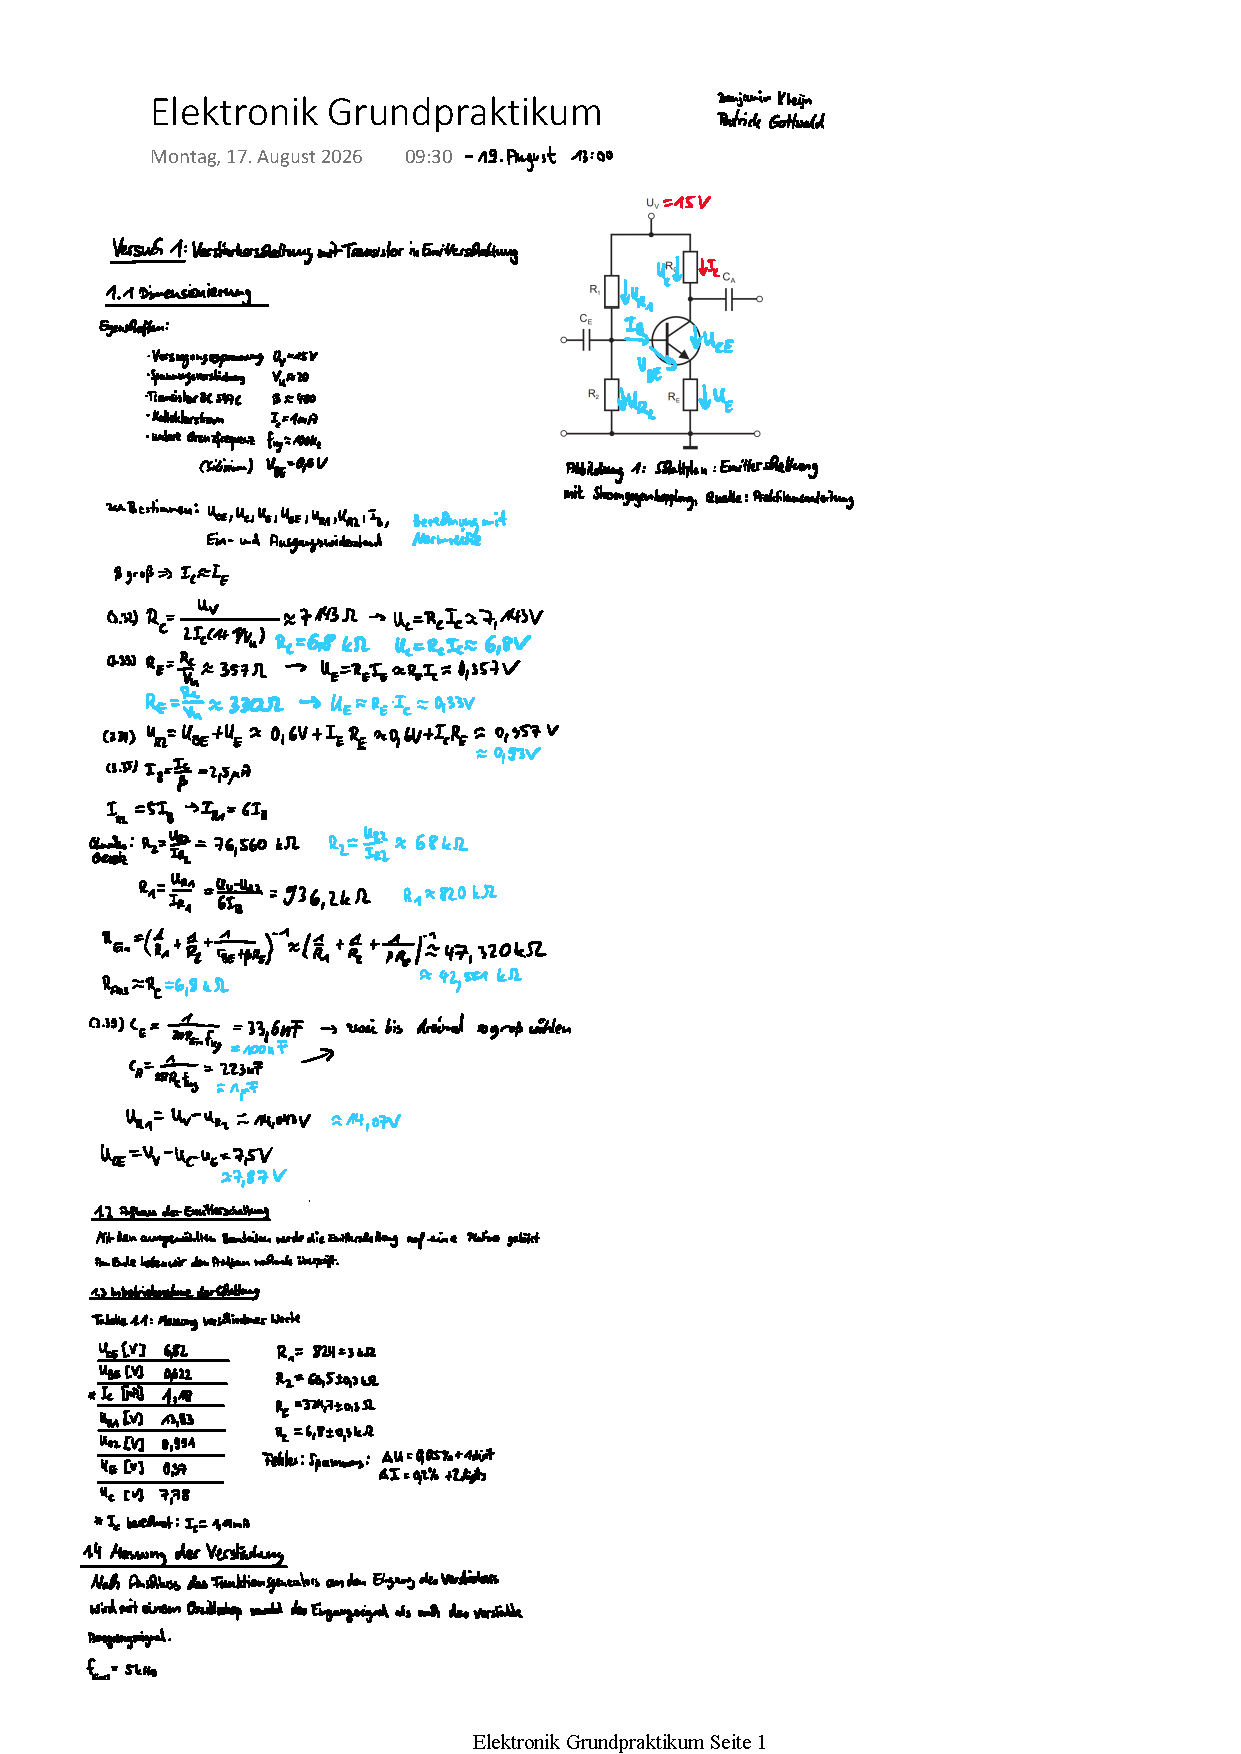
\includepdf[pages=1-7, addtotoc={1, subsection, 2, Messprotokoll, Messprotokoll}]{../../Elektronik Grundpraktikum.pdf}
% % Eigene S-Spalte mit festem Zahlenformat
% \newcolumntype{N}{S[table-format=3.2]}

% \begin{table}[htb]
%   \centering
%   \caption{Dimensionierung der Emitterschaltung}
%   % N ist die Zahl, @{\,} setzt einen kleinen Abstand, l ist die Einheit
%   \begin{tabularx}{0.8\textwidth}{X N @{\,} l N @{\,} l}
%     \toprule
%     Bauteil & \multicolumn{2}{c}{theoretisch} & \multicolumn{2}{c}{Normreihe} \\
%     \midrule
%     $R_C$            &   7.14 & \unit{\kilo\ohm} &   6.80 & \unit{\kilo\ohm} \\
%     $R_E$            & 357.14 & \unit{\ohm}      & 330.00 & \unit{\ohm} \\
%     $R_1$            & 936.19 & \unit{\kilo\ohm} & 820.00 & \unit{\kilo\ohm} \\
%     $R_2$            &  76.57 & \unit{\kilo\ohm} &  68.00 & \unit{\kilo\ohm} \\
%     $C_{\text{EIN}}$ &  33.63 & \unit{\nano\farad}& 100.00 & \unit{\nano\farad} \\
%     $C_{\text{AUS}}$ & 222.82 & \unit{\nano\farad}&   1.00 & \unit{\micro\farad} \\
%     \bottomrule
%   \end{tabularx}
%   \label{table:emitterschaltung}  
% \end{table}
